\documentclass[border=10pt]{standalone}
\usepackage{tikz}
\usetikzlibrary{
    arrows.meta,
    decorations.pathmorphing,
    backgrounds,
    calc
}

\begin{document}
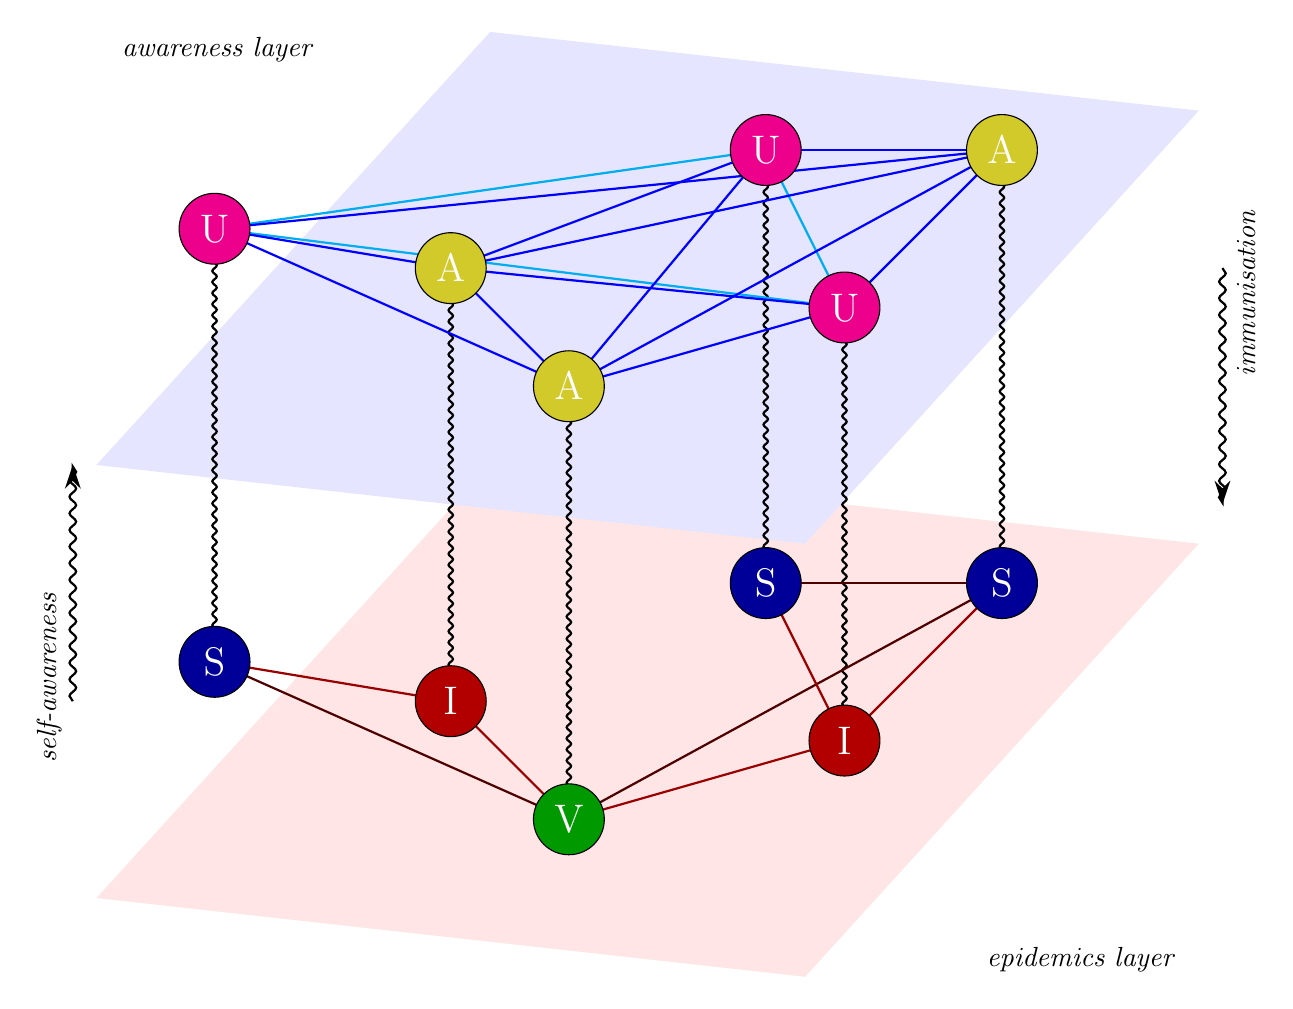
\begin{tikzpicture}[
    % Node styles
    node_style/.style={circle, draw=black, font=\Large, text=white, minimum size=0.9cm, inner sep=0pt},
    U/.style={node_style, fill=magenta},
    A/.style={node_style, fill=yellow!80!black},
    S/.style={node_style, fill=blue!60!black},
    I/.style={node_style, fill=red!70!black},
    V/.style={node_style, fill=green!60!black},
    % Edge styles
    inter_link/.style={decorate, decoration={snake, segment length=4pt, amplitude=0.8pt}, thick},
    wavy_arrow/.style={decorate, decoration={snake, segment length=6pt, amplitude=1.2pt}, -{Stealth[length=3mm, width=2mm]}, thick},
    awareness_link/.style={blue, thick},
    awareness_link_U/.style={cyan, thick},
    epidemics_link_dark/.style={red!60!black, thick},
    epidemics_link_light/.style={red!30!black, thick}
]

% Define vertical separation between layers
\def\layersep{5.5}

% Define coordinates for nodes on the bottom layer
\coordinate (S1) at (-4.5, 0.5);
\coordinate (I1) at (-1.5, 0);
\coordinate (V) at (0, -1.5);
\coordinate (S2) at (2.5, 1.5);
\coordinate (I2) at (3.5, -0.5);
\coordinate (S3) at (5.5, 1.5);

% Define coordinates for nodes on the top layer, shifted vertically
\coordinate (U1) at ($(S1)+(0,\layersep)$);
\coordinate (A1) at ($(I1)+(0,\layersep)$);
\coordinate (A2) at ($(V)+(0,\layersep)$);
\coordinate (U2) at ($(S2)+(0,\layersep)$);
\coordinate (U3) at ($(I2)+(0,\layersep)$);
\coordinate (A3) at ($(S3)+(0,\layersep)$);

% Draw the background planes (parallelograms) on a background layer
\begin{scope}[on background layer]
    \fill[red!10] (-6, -2.5) -- (3, -3.5) -- (8, 2) -- (-1, 3) -- cycle;
    \fill[blue!10] (-6, -2.5+\layersep) -- (3, -3.5+\layersep) -- (8, 2+\layersep) -- (-1, 3+\layersep) -- cycle;
\end{scope}

% Draw inter-layer connections (wavy black lines)
\draw[inter_link] (U1) -- (S1);
\draw[inter_link] (A1) -- (I1);
\draw[inter_link] (A2) -- (V);
\draw[inter_link] (U2) -- (S2);
\draw[inter_link] (U3) -- (I2);
\draw[inter_link] (A3) -- (S3);

% Draw intra-layer connections for the epidemics layer (bottom)
\draw[epidemics_link_light] (S1) -- (V);
\draw[epidemics_link_light] (V) -- (S3);
\draw[epidemics_link_light] (S2) -- (S3);
\draw[epidemics_link_dark] (S1) -- (I1);
\draw[epidemics_link_dark] (I1) -- (V);
\draw[epidemics_link_dark] (V) -- (I2);
\draw[epidemics_link_dark] (I2) -- (S2);
\draw[epidemics_link_dark] (I2) -- (S3);

% Draw intra-layer connections for the awareness layer (top)
% It's a complete graph K6. Edges between U-nodes are cyan, others are blue.
% Cyan links (U-U)
\draw[awareness_link_U] (U1) -- (U2);
\draw[awareness_link_U] (U1) -- (U3);
\draw[awareness_link_U] (U2) -- (U3);

% Blue links (U-A and A-A)
\foreach \source in {U1, U2, U3} {
    \foreach \dest in {A1, A2, A3} {
        \draw[awareness_link] (\source) -- (\dest);
    }
}
\foreach \source/\dest in {A1/A2, A1/A3, A2/A3} {
    \draw[awareness_link] (\source) -- (\dest);
}

% Draw the nodes on top of the edges
% Bottom layer nodes
\node[S] at (S1) {S};
\node[I] at (I1) {I};
\node[V] at (V) {V};
\node[S] at (S2) {S};
\node[I] at (I2) {I};
\node[S] at (S3) {S};
% Top layer nodes
\node[U] at (U1) {U};
\node[A] at (A1) {A};
\node[A] at (A2) {A};
\node[U] at (U2) {U};
\node[U] at (U3) {U};
\node[A] at (A3) {A};

% Add text labels and descriptive arrows
\node[anchor=south west, font=\itshape] at (-5.8, 2.5+\layersep) {awareness layer};
\node[anchor=north east, font=\itshape] at (7.8, -3) {epidemics layer};

\draw[wavy_arrow] (8.3, 5.5) -- (8.3, 2.5);
\node[anchor=west, rotate=90, font=\itshape] at (8.6, 4) {immunisation};

\draw[wavy_arrow] (-6.3, 0) -- (-6.3, 3);
\node[anchor=east, rotate=90, font=\itshape] at (-6.6, 1.5) {self-awareness};

\end{tikzpicture}
\end{document}